% Chapter Template

\chapter{Methods: Stochastic Collocation for Generalized Polynomial Chaos} % Main chapter title

\label{ch:methods scgpc} % Change X to a consecutive number; for referencing this chapter elsewhere, use \ref{ChapterX}

\lhead{Chapter 2. \emph{Methods: Collocation for Polynomial Chaos}} % Change X to a consecutive number; this is for the header on each page - perhaps a shortened title

%----------------------------------------------------------------------------------------
%	SECTION: INTRO
%----------------------------------------------------------------------------------------

\section{Introduction}
In this chapter we describe several common and novel uncertainty quantification methods and their applications.
We begin
by discussing the principles of input spaces and responses, and define terminology used in this work.  Next we
discuss uncertainty quantification at a high level, and describe several common uncertainty quantification
tools.  Finally, we explore Stochastic Collocation for generalized Polynomial Chaos (SCgPC), an advanced
uncertainty quantification technique.

% inputs and outputs
Many simulation models are algorithms constructed to solve partial differential equations, often in two or
three spatial dimensions and possibly time.  The inputs to these models include boundary conditions, material
properties, tuning parameters, and so forth.  The outputs are responses, either data fields or
scalar values.  The responses are used to inform decision-making processes.  For example, a neutronics
simulation in nuclear engineering takes materials, geometries, and boundary conditions as inputs, and yields
neutron flux and the neutron multiplication factor $k$ as responses.  Similarly, a fuels performance code
takes materials, geometries, and power shapes as inputs and yields stresses, strains, and temperature profiles
as outputs.  Figure \ref{fig:ober} is an example of this workflow \cite{oberkampf}.
\begin{figure}
  \centering
  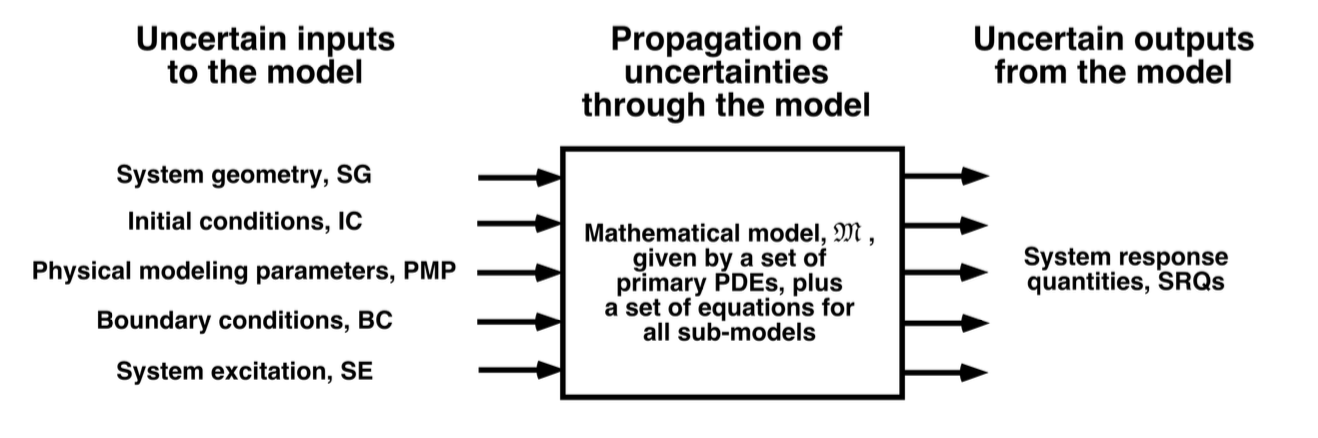
\includegraphics[width=\linewidth]{v_and_v_uq}
  \caption{Uncertainty Quantification \cite{oberkampf}}
  \label{fig:ober}
\end{figure}

In general, we define $u(Y)$ to be
a response as a function of the input space $Y = (y_1,\ldots,y_n,\ldots,y_N)$ where $y_n$ is a single
uncertain input
parameter to the model, $n$ is an index spanning the number of inputs, and $N$ is the total number of inputs.
Uncertain input parameters can include any of the inputs to the simulation.
We assume each response to be a scalar, integrated quantity.  In the event
the output is a vector or field quantity, each element can be considered as a distinct scalar response.
\emph{Models} are mathematical equations used to obtain the response $u(Y)$, and \emph{solvers} or
\emph{simulations} are numerical algorithms used to solve models.

Using our examples above, for neutronics calculations $Y$ might include nuclear cross sections, geometry
parameters, and sources, while $u(Y)$ could be $k$-effective or the neutron flux at a particular location of
interest.  For fuels performance calculations, $Y$ might entail thermal conductivity of various parameters,
geometric construction parameters, moderator inlet temperatures, and so forth.  $u(Y)$ could be peak clad
temperature, maximum fuel centerline temperature, clad elongation, percent fission gas released, and so on.

\subsection{Uncertain Inputs}
Essential to using simulation models is understanding the possibility that significant uncertainties existing in
the inputs.  These could be aleatoric uncertainties due to intrinsic randomness in the inputs, or epistemic
uncertainties due to model imperfections or lack of knowledge.  
For example, quantum behaviors or Brownian motion often provide non-deterministic sources of aleatoric uncertainty.
Further, the simulation itself might be solved through non-deterministic methods such as Monte Carlo sampling,
in which case the random seed acts as an uncertain input.  Examples of epistemic uncertainties include initial
or boundary conditions that can only be controlled to some finite level, such as manufacturing tolerances,
temperature and pressure, and so forth.
Each of these aleatoric and epistemic uncertainties has some
distribution defining the likelihood of an input to have a particular value.  Sometimes these distributions
are known; often, they can only be approximated.  These distributions might be
assumed or constructed from experiment; for our work, we will assume distributions are given, and that the given 
distributions are accurate.  The
input likelihood distribution is the probability distribution function (PDF) $\rho_n(y_n)$.  
An integral over any portion of the input space of the PDF provides the probability that the input's value
is within that portion.
We require
\begin{equation}
  \int_a^b \rho_n(y_n) d\ y_n = 1,
\end{equation}
where $a$ and $b$ are the minimum and maximum values $y_n$ can take (possibly infinite).  In other words, the
probability of finding the input between $a$ and $b$ is 100\%; similarly, we can say the value of the input
lies between $a$ and $b$ almost surely.

\subsection{Multidimensional Input Spaces}
% multidimensional
When there are more than one uncertain input, the combination of distributions for these inputs span an
uncertainty space $\Omega$. $\Omega$ is a part of the probability space $(\Omega,\sigma,\rho)$, where $\Omega$
is the set of all possible outcomes, $\sigma$ is the set of events $\omega$, and $\rho$ is the probability function for
the space.  The dimensionality of $\Omega$ is $N$,
the number of uncertain input variables.  The probability of any event in the input space occurring is given
by an integral of the joint-probability distribution $\rho(Y)$, still enforcing
\begin{equation} \label{eq:joint pdf}
  \int_{a_1}^{b_1}\cdots\int_{a_N}^{b_N} \rho(Y) dy_1\cdots dy_N = 1.
\end{equation}
For clarity, we define multidimensional integral operator
\begin{equation}
  \int_\Omega (\cdot)dY\equiv \int_{a_1}^{b_1}\cdots\int_{a_N}^{b_N} (\cdot) dy_1\cdots dy_N,
\end{equation}
so that Eq. \ref{eq:joint pdf} can be written
\begin{equation}
  \int_\Omega \rho(Y) dY = 1.
\end{equation}
The function $u(Y)$ maps realizations ($\omega$) from the input space $\Omega$ to a real-valued response.
That is, for each input variable $y_n$, a realization is taken by selecting a single value from the
distribution of $y_n$, which gives a single input value $y_n(\omega)$.  Taking a single realization of each of
the distributed input parameters yields a full input realization $Y(\omega)=(y_1(\omega),\cdots,y_N(\omega))$,
which can be used as inputs for
$u(Y)$ to obtain a realization of the response $u(Y(\omega))$.  To simplify notation, in general the
dependency of a realization on $\omega$ will be omitted and referred to as \emph{sampling} or \emph{taking a
realization}.

% correlation
\subsection{Correlation and the Karhunen-Loevre expansion}\label{sec:kl}
We note the possibility that multiple inputs may be correlated with each other.  When inputs are not
independent, the joint probability distribution is not the product of each individual probability distribution
distribution.  When this is the case, each distribution cannot be sampled independently, and this
creates complications for many of the sampling strategies presented in this work.  

Using input space mapping, however, a surrogate orthogonal input space can be
constructed.  This surrogate space is functionally identical to the original for our purposes.
There are mathematical approaches to decoupling input parameters through surrogate
spaces.  In particular, using principle component analysis (or Karhunen-Loeve expansion
\cite{karhunen} for discrete inputs), the covariance matrix for the distributed input parameters
can be used to construct a multidimensional
standard Gaussian normal distribution, whose components are all orthogonal.
As a result, we only consider independent variables in this work, as dependent variables can
be decoupled through this surrogate mapping process.


\section{Uncertainty Quantification}
% introduction
The purpose of uncertainty quantification is to propagate the uncertainties present in the input space of a
problem through the model and comprehend their effects on the output responses.  In traditional simulations, a
single value for each input variable results in a single value for the response.  When performing uncertainty
quantification, a range of values for each input results in a range of response values.  To quantify the
distribution of the output response, often statistical moments are used, including the mean, variance,
skewness, and kurtosis.
\subsection{Statistical Moments}
The mean provides the expected value of the response, or generally the most probable
value for the response.  The variance establishes the spread of the response, or the distance response values
have from the mean on average.  The standard deviation of the response is given by the square root of the
variance, and provides a useful metric to determine the probability of finding a response value within a
range.  For instance, Chebyshev's inequality \cite{chebyshevineq} says $1-1/k^2$ of a distribution's values
are within $k$ standard deviations from the mean.  This is true whenever the mean and variance can be
defined.  Table
\ref{tab:cheby stdev} shows the minimum percent of the response covered by expanding the range by multiples of the
standard deviation.
Some distributions are much more restrictive than Chebyshev's inequality requires.  For instance, we 
show a similar table for a normal Gaussin distribution in Table \ref{tab:norm stdev}.  Fig. \ref{fig:stdev pct}
shows the same information graphically.
\begin{table}[htb]
  \centering
  \begin{tabular}{c c}
  Number of Std. Dev. & Percent of Values \\ \hline
  1 & 0 \\
  $\sqrt{2}$ & 50 \\
  2 & 75 \\
  3 & 88.89 \\
  4 & 93.75 \\
  5 & 96 \\
  10 & 99
  \end{tabular}
  \caption{Percentage of Values within $k$ standard deviations for general distributions}
  \label{tab:cheby stdev}
\end{table}
\begin{table}[htb]
  \centering
  \begin{tabular}{c c}
  Number of Std. Dev. & Percent of Values \\ \hline
  1 & 68.3 \\
  2 & 95.45 \\
  3 & 99.73 \\
  4 & 99.994 \\
  \end{tabular}
  \caption{Percentage of Values within $k$ standard deviations for Gaussian normal}
  \label{tab:norm stdev}
\end{table}
\begin{figure}[H]
  \centering
  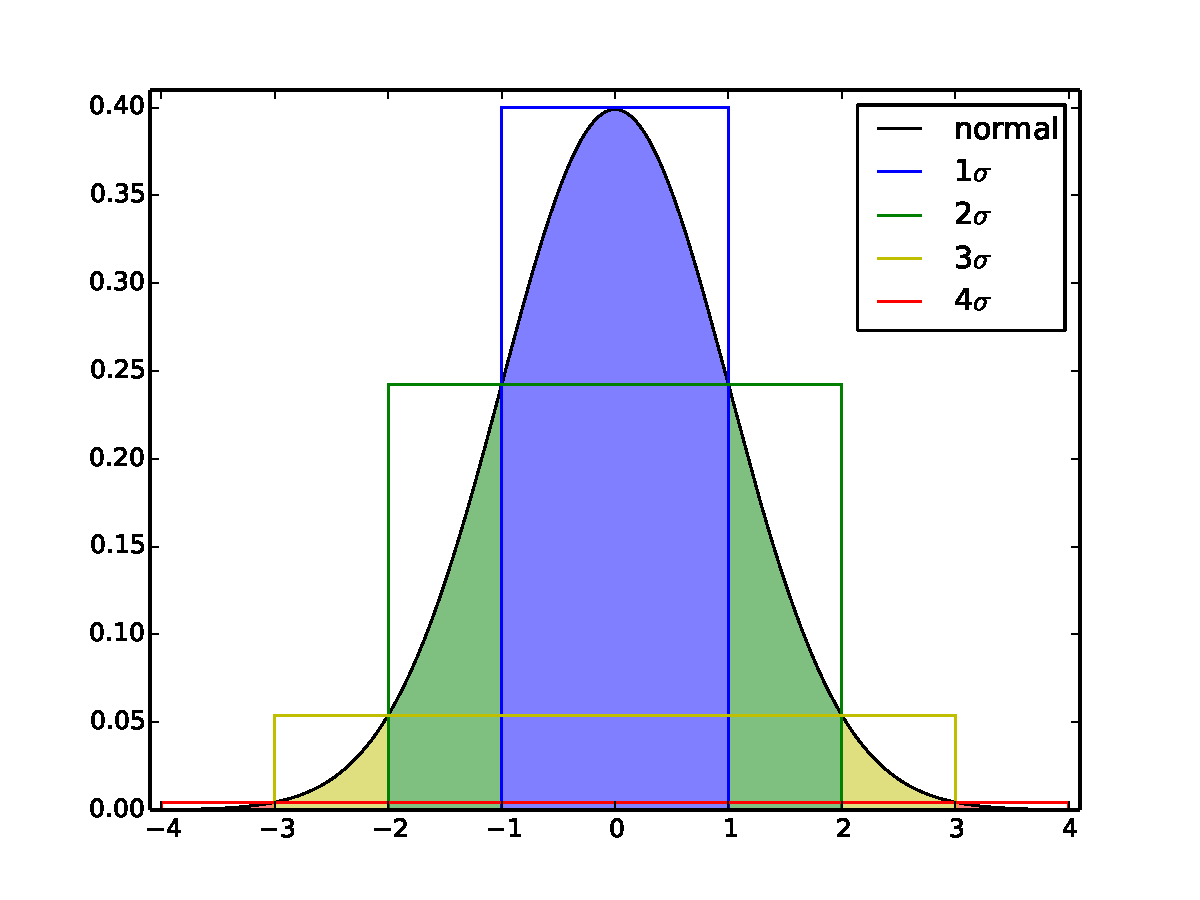
\includegraphics[width=0.7\linewidth]{stdev_pct}
  \caption{Standard Deviations of Normal Gaussian Distribution}
  \label{fig:stdev pct}
\end{figure}
Higher order moments, skewness and kurtosis, describe the asymmetry and "tailedness"
of the response distribution respectively.  The more asymmetric the distribution, the
higher the skewness is.  For example, a Gaussian normal distribution has zero skewness,
and skewness is introduced to a Beta distribution by allowing $\alpha\neq\beta$.
Kurtosis is more complicated in its interpretation, but in general kurtosis provides an idea
of how much of the variance is contributed by extreme deviations from the mean.  The kurtosis
of a Guassian normal distribution is 3.  This leads to the definition of excess kurtosis,
which is 3 less than the traditional kurtosis.

While both the skewness and kurtosis provide insight as to the distribution of reponses,
most uncertainty quantification is centered on second-order metrics.
Second-order uncertainty quantification seeks for the mean and variance of
the perturbed response.  Mathematically, the mean of a model is the first moment,
\begin{equation}
  \text{mean} = \expv{u(Y)} = \int_\Omega \rho(Y) u(Y) dY,
\end{equation}
and the variance is the second moment less the square of the first,
\begin{equation}
  \text{variance} = \expv{u(Y)^2} - \expv{u(Y)}^2 = \int_\Omega \rho(Y) u(Y)^2 dY - \text{mean}^2.
\end{equation}
 
Another use for uncertainty quantification is understanding the sensitivity of the output responses to the
uncertain inputs; that is, determining how responses change as a function of changes in the input space.  At
the most primitive level, linear sensitivity of a response mean to an input is the derivative of the response
with respect to the input.  Sensitivities can be both local to a region in the input space as well as global
to the entire problem.

In addition, there are two chief methods to define sensitivity.  One of the most typical sensitivities
is mean to mean; that is, the rate of change in the value of the reponse as a function of changes in the
input.  This metric is most useful what attempting to maximize or minimize a response value by changing
input parametrs.  The second method is variance to variance, or the rate of change in the variance of the
response as a function of changes in the variance of an input.  This is useful when trying to mitigate the
spread of possible response values.  If there is a possibility of a response having an undesirable value,
knowing the variance-variance sensitivity helps in identifying which inputs need to have their variance
reduced to prevent the undesirable value from occuring.

\subsection{After Uncertainty Quantification}
Once the response distribution is well-understood through statistical moments and sensitivities, 
further analysis
and decisions can be made.  For example, one post-uncertainty quantification analysis is limit
surface definition and failure probability.  In this analysis, a criteria is given that determines
a ``success'' and ``failure'' condition for a response.  For instance, in the simulation of a
material undergoing stress during heating, a failure condition could be whether the material
buckles during the simulation.  The limit surface search seeks to determine what portion of the
input space leads to failures, and what portion to successes, and define the hypersurfaces dividing
successes and failures.  After a limit surface search, optimization can be performed, which gives
some criteria for ideal operation and searches the success space for optimal inputs.  For example,
if alloy compositions are the inputs for the stress and heat material mentioned earlier, optimization
can help find the least expensive alloy that won't buckle in the conditions given by the simulation.

Another post-uncertainty quantification calculation is to make use of sensitivity information to determine
the inputs that could benefit from reduced variance to reduce the variance of the response in turn.
If some inputs have minimal impact on variance in the output, they don't need the same level of care
in manufacturing as other inputs.  For example, consider the construction of a commercial nuclear power
reactor.  If the material properties and geometry of the reflector have a much smaller impact on the operation
variance than the fuel content and geometry of the fuel pellets, the most naieve cost-effective way to control
variance are to decrease margins in fuel manufacturing instead of reflector construction.  While this example
seems readily evident, often engineering intuition can be surprised by uncertainty quantification and
sensitiviy analysis.

\subsection{Analytic Uncertainty Quantification}
For some models, there exists analytic techniques for propagation of uncertainty.  One of these is the
so-called \emph{sandwich formula}, often referred to as \emph{standard propagation of error} \cite{sandwich}.
Assuming independent input parameters (see section \ref{sec:KL}), the standard deviation $\sigma_u$ of $u(Y)$
is given as
\begin{equation}
  \sigma^2_u = \sum_{n=1}^N \qty(\pdv{u(Y)}{y_n})^2\sigma_{y_n}^2,
\end{equation}
where $\sigma_{y_n}$ is the standard deviation of uncertain input $y_n$.  This approximation is limited to the
linear characteristics of the gradient of $u(Y)$, and so is useful especially when the standard deviation of
the inputs are small compared to the partial derivatives \cite{sandwich2}.

For models with gradients that are simple to calculate accurately (and sufficiently small input
uncertainties), this formula is very effective at propagating error.  However, computing or estimating such
gradients accurately for complex models is prohibitive, and leads to numerical approaches to uncertainty
quantification, as we discuss in this thesis.


\subsection{Uncertainty Quantification Techniques}
There are several common tools used for uncertainty quantification when analytic analysis is not possible.
These include stochastic methods such as Monte Carlo sampling, deterministic methods such as Grid sampling,
and mixed methods such as Latin Hypercube sampling (LHS).  After describing these, we also consider advanced
uncertainty quantification techniques: generalized polynomial chaos expansion and high-dimension
model reduction.

\subsection{Monte Carlo}
The Monte Carlo method \cite{mc} has been used formally since the 1930s as a tool to explore possible outcomes
in uncertain models.  Nuclear physicist Enrico Fermi used the method in his work with neutron moderation in
Rome \cite{mcfermi}.  In its simplest form, Monte Carlo involves randomly picking realizations from a set of
possibilities, then statistically collecting the results.  In uncertainty quantification, Monte Carlo can be
used to sample points in the input space based on the joint probability distribution.  The collection of
points is analyzed to determine the moments of the response.

The mean of a response is determined using the unweighted average of samples collected:
\begin{equation}
  \expv{u(Y)} = \frac{1}{N}\sum_{m=1}^M \qty(u(Y_m)) + \epsilon_M^{\text{MC}},
\end{equation}
where $Y_m$ is a realization randomly chosen based on $\rho(Y)$, and $M$ is the total number of samples taken.
The error in the approximation diminishes with the root of the number of samples taken,
\begin{equation}
  \epsilon_M^{\text{MC}} \propto \frac{1}{\sqrt{M}}.
\end{equation}
The second moment is similarly approximated as
\begin{equation}
  \expv{u(Y)^2} \approx \frac{1}{N}\sum_{m=1}^M \qty(u(Y_m)^2).
\end{equation}
The standard deviation (root of the variance) converges similarly to the mean for Monte Carlo methods.  There
are many tools that can be used to improve Monte Carlo sampling \cite{mcvarred}\cite{mcnpvarred}; we restrict
our discussion to traditional analog Monte Carlo sampling.

Monte Carlo has long been a gold standard for uncertainty quantification because of its consistency.  Monte
Carlo will always resolve the response statistics given a sufficient number of samples.  Additionally, the
convergence of Monte Carlo is largely agnostic of the input space dimensionality, a feature not shared by the
LHS and Grid sampling methods.

The drawback to Monte Carlo sampling also centers on its consistency.  The error in analog Monte Carlo can only be
consistently reduced by drastically increasing the number of samples calculated.  While coarse estimates are
inexpensive to obtain, high precision takes a great deal of runs to converge.

TODO 2d, 3d grid example

\subsection{Grid}
One of the drawbacks of Monte Carlo is lack of control over points sampled.  While LHS can improve this
somewhat, another alternative is using a structured orthogonal grid.  In this strategy, the input space is
divided into hypervolumes that are equal in volume either in the input space or in uncertainty space.  For
demonstration, we first consider a one-dimensional case with a single normally-distributed variable $y$ with mean
$\mu$ and standard deviation $\sigma$.  If the input space is divided into equal volumes in the input space, a lower and upper bound are determined,
then nodes are selected on the ends and equally spaced throughout.  See Figure TODO.  If the input space is
divided into equal probability volumes, nodes are selected to be equidistant along the cumulative distribution
function (CDF).  This assures that the volume between each set of nodes has equal probability.  See Figure TODO.
TODO Figure should show both equal spacing and CDF spacing, plus a normal distribution for comparison.
In higher dimensions, a grid is constructed as a tensor product of each grid.

Since the grid nodes are user-defined, approximating integrals are slightly more complicated than in the Monte
Carlo space.  The mean is approximated by
\begin{equation}
  \expv{u(Y)} = \int_\Omega \rho(Y) u(Y) dY \approx \sum_{m=1}^M w_m u(Y_m),
\end{equation}
where $m$ iterates over each node in the grid, $Y_m$ is the multidimensional input point as node $m$, and
$w_m$ is a probability weight determined by the volume of probability represented by the node.  In grids
constructed by CDF, all $w_m$ are of the same value, while in grids spaced equally by value, $w_m$ can vary
significantly.  Similarly, the second moment is approximated by
\begin{equation}
  \expv{u(Y)^2} = \int_\Omega \rho(Y) u(Y)^2 dY \approx \sum_{m=1}^M w_m u(Y_m)^2.
\end{equation}

An advantage to grid sampling is its regular construction, which can give more clarity to how a response
behaves throughout the input space.  However, the grid construction suffers greatly from the curse of
dimensionality, which makes it inefficient for input spaces with large dimensionality. TODO references
TODO 2d, 3d grid example

\subsection{LHS}
A cross between Monte Carlo and Grid sampling strategies, the Latin Hypercube Sampling (LHS) strategy 
has long been a sampling tool used to reduce
the total samples needed without significantly sacrificing integration quality \cite{lhs}.  In LHS, the input
space is also divided into a grid just as in the Grid sampling strategy.  However, unlike Grid sampling, only
one sample is taken per hyperplane; that is, for any of the input variables, there is only one sample taken
between each of the one-dimensional nodes.  Once a hypervolume is selected to take a sample, the exact
point is selected by random sampling in the probability space within the hypervolume.  See for example the
sampling in Figure TODO.

As in the Grid method, the weight of each sample is the probability volume of the hypervolume it represents.

\section{Generalized Polynomial Chaos}
Expanding beyond the traditional uncertainty quantification methods of Monte Carlo, Grid, and LHS sampling, there are more
advanced methods that are quite efficient in particular applications.
Polynomial chaos expansion (PCE) methods, for example, seek to interpolate the simulation code as a combination of
polynomials of varying degree in each dimension of the input space.  There are several advantages to expanding
in polynomials.  TODO citation!  First, orthonormal polynomials have means and standard deviations that are trivial to calculate
analytically, even for computer algorithms.  Second, the resulting polynomial expansion is an
inexpensive surrogate model that can be used in place of the original.  Third, the unknowns in the expansions
are scalar coefficients, which can often be efficiently calculated through numerical integration.

Originally Wiener
proposed expanding in Hermite polynomials for Gaussian-normal distributed variables \cite{wiener}.  Askey and
Wilson generalized Hermite polynomials to include Jacobi polynomials, including Legendre and Laguerre
polynomials \cite{Wiener-Askey}.  Xiu and Karniadakis combined these concepts to perform PCE for a range of Gaussian-based
distributions with corresponding polynomials,
including Legendre polynomials for uniform distributions, Laguerre polynomials for Gamma distributions, and
Jacobi polynomials for Beta distributions \cite{xiu}.

In each of these cases, a probability-weighted
integral over the distribution can be cast in a way that the corresponding polynomials are orthogonal over the
same weight and interval.  These chaos Wiener-Askey polynomials were used by Xiu and Karniadakis to develop
the generalized polynomial chaos expansion method (gPC), including a transformation for applying the same
method to arbitrary distributions (as long as they have a known inverse CDF) \cite{xiu}.  Two significant
methodologies have grown from gPC application.  The first makes use of Lagrange polynomials to expand the
original function or simulation code, as Lagrange polynomials can be made orthogonal over the same domain as the
distributions \cite{SCLagrange}; the other uses the Wiener-Askey polynomials \cite{xiu}.  We consider the latter in this work.

We consider a simulation code that produces a quantity of interest $u$ as a function $u(Y)$ whose arguments are
the uncertain, distributed input
parameters $Y=(Y_1,\ldots,Y_n,\ldots,Y_N)$.  A particular realization $\omega$ of $Y_n$ is expressed by
$Y_n(\omega)$, and a single realization of the entire input space results in a solution to the function as
$u(Y(\omega))$.  We acknowledge obtaining a realization of $u(Y)$ may take considerable computation time and
effort, and may be solved nonlinearly.  There also may be other input parameters that
contribute to the solution of $u(Y)$; we neglect these, as our interest is in the uncertainty space; all
parameters without uncertainty are held at their nominal values.
In addition, it is possible that the quantity of interest $u(Y)$ is an integrated quantity or some norm of a
value that is temporally or spatially distributed. We restrict $u(Y(\omega))$ to a single scalar
output, but the same principles apply to a multidimensional response.  Further, a quantity of interest may be
time-dependent in a transient simulation.  In this case, the PCE can be constructed at several selected points
in time throughout the simulation, which can then be interpolated between.  In effect, the polynomial
coefficients become time-dependent scalar values.  For now, we consider a static case with no time dependence.

We expand $u(Y)$ in orthonormal multidimensional polynomials $\Phi_k(Y)$, where $k$ is a multi-index tracking
the polynomial order in each axis of the polynomial Hilbert space, and $\Phi_k(Y)$ is constructed as
\begin{equation}\label{eq:gPC}
  \Phi_k(Y) = \prod_{n=1}^N \phi_{k_n}(Y_n),
\end{equation}
where $\phi_{k_n}(Y_n)$ is a single-dimension Wiener-Askey orthonormal polynomial of order $k_n$ and
$k=(k_1,\ldots,k_n,\ldots,k_N)$, $k_n\in\mathbb{N}^0$.  For example, given $u(y_1,y_2,y_3)$, $k=(2,1,4)$
is the multi-index of the
product of a second-order polynomial in $y_1$, a first-order polynomial in $y_2$, and a fourth-order
polynomial in $y_4$. The gPC for $u(Y)$ using this notation is
\begin{equation}
  u(Y) \approx \sum_{k\in\Lambda(L)} u_k\Phi_k(Y),
\end{equation}
where $u_k$ is a scalar weighting polynomial coefficient. The polynomials used in the expansion are determined
by the set of multi-indices $\Lambda$, which can be selected in a variety of ways we will discuss in section
\ref{sec:index sets} and are the essence of this work.  In the limit
that $\Lambda$ contains all possible combinations of polynomials of any order, Eq. \ref{eq:gPC} is exact.
Practically, however, $\Lambda$ is truncated to some finite set of combinations, discussed in section
\ref{sec:index sets}.

Using the orthonormal properties of the Wiener-Askey polynomials,
\begin{equation}
  \int_\Omega \Phi_k(Y)\Phi_{\hat k}(Y) \rho(Y) dY = \delta_{k\hat k},
\end{equation}
where $\rho(Y)$ is the combined PDF of $Y$, $\Omega$ is the multidimensional domain of $Y$, and $\delta_{nm}$
is the Dirac delta, we can isolate an expression for the polynomial expansion coefficients.
We multiply both sides of Eq. \ref{eq:gPC} by
$\Phi_{\hat k}(Y)$, integrate both sides over the probability-weighted input domain, and sum over all $\hat k$
to obtain the coefficients, sometimes referred to as polynomial expansion moments,
\begin{align}\label{eq:polycoeff}
  u_k &= \frac{\langle u(Y)\Phi_k(Y) \rangle}{\langle \Phi_k(Y)^2 \rangle},\\
      &= \langle u(Y)\Phi_k(Y) \rangle,
\end{align}
where we use the angled bracket notation to denote the probability-weighted inner product,
\begin{equation}
  \langle f(Y) \rangle \equiv \int_\Omega f(Y)\rho(Y) dY.
\end{equation}
When $u(Y)$ has an analytic form, these coefficients can be solved by integration; however, in general other
methods must be applied to numerically perform the integral.  While tools such as Monte Carlo integration can
be used to evaluate the integral, we can harness the properties of Gaussian quadratures because of the
probability weights and domain.  This stochastic collocation method is discussed in section \ref{sec:stoch
coll}.

\subsection{Polynomial Index Set Construction}\label{sec:index sets}
The chief concern in expanding a function in interpolating multidimensional polynomials is choosing appropriate polynomials to
make up the expansion.
There are many generic ways by which a polynomial set can be constructed.  Here we present three static
approaches: tensor
product, total degree, and hyperbolic cross.

In the nominal tensor
product case, $\Lambda(L)$ contains all possible combinations of polynomial indices up to truncation order $L$ in each
dimension, as
\begin{equation}
  \Lambda_\text{TP}(L)=\Big\{\bar p=(p_1,\cdots,p_N): \max_{1\leq n\leq N}p_n\leq L
\Big\}.
\end{equation}
The cardinality of this index set is $|\Lambda_\text{TP}(L)|=(L+1)^N$. For example, for a two-dimensional
input space ($N$=2) and truncation limit $L=3$, the index set $\Lambda_\text{TP}(3)$ is given in Table
\ref{tab:TP}, where the notation $(1,2)$ signifies the product of a polynomial that is first order in $Y_1$
and second order in $Y_2$.

\begin{table}[h]
  \centering
  \begin{tabular}{c c c c}
    (3,0) & (3,1) & (3,2) & (3,3) \\
    (2,0) & (2,1) & (2,2) & (2,3) \\
    (1,0) & (1,1) & (1,2) & (1,3) \\
    (0,0) & (0,1) & (0,2) & (0,3)
  \end{tabular}
  \caption{Tensor Product Index Set, $N=2,L=3$}
  \label{tab:TP}
\end{table}

It is evident there is some inefficiencies in this index set.  First, it suffers dramatically from the
\emph{curse of dimensionality}; that is, the number of polynomials required grows exponentially with
increasing dimensions.  Second, the total order of polynomials is not considered.  Assuming the contribution of
each higher-order polynomial is smaller than lower-order polynomials, the (3,3) term is
contributing sixth-order corrections that are likely smaller than the error introduced by ignoring
fourth-order corrections (4,0) and (0,4).  This leads to the development of the \emph{total degree} (TD) and
\emph{hyperbolic cross} (HC) polynomial index set construction strategies \cite{hctd}.

In TD, only multidimensional polynomials whose \emph{total} order at most $L$ are permitted,
\begin{equation}
  \Lambda_\text{TD}(L)=\Big\{\bar p=(p_1,\cdots,p_N):\sum_{n=1}^N p_n \leq L
\Big\}.
\end{equation}
The cardinality of this index set is $|\Lambda_\text{TD}(L)|={L+N\choose N}$, which grows with increasing
dimensions much more slowly than TP.  For the same $N=2,L=3$ case above, the TD index set is given in Table
\ref{tab:TD}. 

\begin{table}[h]
  \centering
  \begin{tabular}{c c c c}
    (3,0) &       &       &       \\
    (2,0) & (2,1) &       &       \\
    (1,0) & (1,1) & (1,2) &       \\
    (0,0) & (0,1) & (0,2) & (0,3)
  \end{tabular}
  \caption{Total Degree Index Set, $N=2,L=3$}
  \label{tab:TD}
\end{table}

In HC, the \emph{product} of polynomial orders is used to restrict allowed polynomials in the index set.  This
tends to polarize the expansion, emphasizing higher-order polynomials in each dimension but lower-order
polynomials in combinations of dimensions, as
\begin{equation}
  \Lambda_\text{HC}(L)=\Big\{\bar p=(p_1,\ldots,p_N):\prod_{n=1}^N p_n+1 \leq L+1
\Big\}.
\end{equation}
The cardinality of this index set is bounded by $|\Lambda_\text{HC}(L)|\leq (L+1)(1+\log(L+1))^{N-1}$. It
grows even more slowly than TD with increasing dimension, as shown in Table \ref{tab:HC} for $N=2,L=3$.

\begin{table}[h]
  \centering
  \begin{tabular}{c c c c}
    (3,0) &       &       &       \\
    (2,0) &       &       &       \\
    (1,0) & (1,1) &       &       \\
    (0,0) & (0,1) & (0,2) & (0,3)
  \end{tabular}
  \caption{Hyperbolic Cross Index Set, $N=2,L=3$}
  \label{tab:HC}
\end{table}

It has been shown that the effectiveness of TD and HC as index set choices depends strongly on the regularity
of the responce \cite{hctd}.  TD tends to be most effective for infinitely-continuous response surfaces,
while HC is more effective for surfaces with limited smoothness or discontinuities.

\subsection{Anisotropy}
While using TD or HC to construct the polynomial index set combats the curse of dimensionality present in TP,
it is not eliminated and continues to be an issue for problems of large dimensionality.  Another method that can
be applied to mitigate this issue is index set anisotropy, or the unequal treatment of various dimensions.
In this strategy, weighting factors $\alpha=(\alpha_1,\ldots,\alpha_n,\ldots,\alpha_N)$ are applied in each
dimension to allow additional polynomials in some dimensions and less in others.  This change adjusts the TD
and HC construction rules as follows, where $|\alpha|_1$ is the one-norm of $\alpha$.
\begin{equation}
  \tilde\Lambda_\text{TD}(L)=\Big\{\bar p=(p_1,\cdots,p_N):\sum_{n=1}^N \alpha_n p_n \leq \qty|\vec\alpha|_1 L
\Big\},
\end{equation}
\begin{equation}
  \tilde\Lambda_\text{HC}(L)=\Big\{\bar p=(p_1,\cdots,p_N):\prod_{n=1}^N \qty(p_n+1)^{\alpha_n} \leq
  \qty(L+1)^{\qty|\vec\alpha|_1} \Big\}.
\end{equation}
As it is desirable to obtain the isotropic case from a reduction of the anisotropic cases, we define the
one-norm for the weights as
\begin{equation}
  |\alpha|_1 = \frac{\sum_{n=1}^N \alpha_n}{N}.
\end{equation}
Considering the same case above ($N=2,L=3$), we apply weights $\alpha_1=5,\alpha_2=3$, and the resulting index
sets are Tables \ref{tab:aniTD} (TD) and \ref{tab:aniHC} (HC).

\begin{table}[h]
  \centering
  \begin{tabular}{c c c c c}
    (2,0) &       &       &       & \\
    (1,0) & (1,1) & (1,2) &       & \\
    (0,0) & (0,1) & (0,2) & (0,3) & (0,4)
  \end{tabular}
  \caption{Anisotropic Total Degree Index Set, $N=2,L=3$}
  \label{tab:aniTD}
\end{table}

\begin{table}[h]
  \centering
  \begin{tabular}{c c c c}
    (1,0) &       &       &       \\
    (0,0) & (0,1) & (0,2) & (0,3)
  \end{tabular}
  \caption{Anisotropic Hyperbolic Cross Index Set, $N=2,L=3$}
  \label{tab:aniHC}
\end{table}

There are many methods by which anisotropy weights can be assigned.  Often, if a problem is well-known to an 
analyst, it may be enough to use heuristics to assign importance arbitrarily.  Otherwise, a smaller
uncertainty quantification solve can be used to roughly determine sensitivity coefficients (such as Pearson
coefficients), and the inverse of those can then be applied as anisotropy weights.  Sobol sensitivity coefficients
 could also serve as a basis for these weights.
A good choice of anisotropy weight can greatly speed up convergence; however, a
poor choice can slow convergence considerably, as computational resources are used to resolve low-importance
dimensions.


\subsection{Polynomial Expansion Features}
As previously mentioned, there are several benefits to the PCE once constructed.  First, the PCE is a
surrogate model for the original response, and can be used in its place as long as all the inputs are within
the same bounds as when the original PCE was constructed.  The error in this representation will be of the
same order as the truncation error of the expansion.

Second, the first and second moments of the PCE are very easy to obtain.  Because the probability-weighted 
integral of all the orthonormal polynomials is zero with the exception of the zeroth-order polynomial, and
using the notation 
\begin{equation}
  u(Y) \approx \tilde u(Y) \equiv \sum_{k\in\lambda} u_k\Phi_k(Y),
\end{equation}
the mean is simply
\begin{align}
  \expv{\tilde u(Y)}  &= \int_\Omega \rho(Y) \sum_{k\in\Lambda} u_k\Phi_k(Y) dY, \nonumber\\
                      &= u_{(0,\cdots,0)}.
\end{align}
The second moment is similarly straightforward.  The integral of the square of the PCE involves cross-products of
all the expansion terms; however, because the integral of the product of any two polynomials is the dirac
delta $\delta_{i,j}$, this simplifies to the sum of the squares of the expansion coefficients,
\begin{align}
  \expv{\tilde u(Y)^2} &=\int_\Omega \rho(Y) \qty[\sum_{k\in\Lambda} u_k\Phi_k(Y)]^2 dY,
                 \nonumber\\ \vspace{5pt}
  &= \int_\Omega \rho(Y) \sum_{k_1\in\Lambda} \sum_{k_2\in\Lambda} u_{k_1}\Phi_{k_1}(Y) \cdot 
                           u_{k_2}\Phi_{k_2}(Y) dY, \nonumber \\ \vspace{5pt}
  &= \sum_{k_1\in\Lambda} \sum_{k_2\in\Lambda} u_{k_1} \cdot u_{k_2}\delta_{k_1,k_2},\nonumber \\ \vspace{5pt}
  &= \sum_{k\in\Lambda} u_k^2.
\end{align}

\section{Stochastic Collocation}\label{sec:stoch coll}
Having outlined the PCE construction and its uses, we turn to the method of calculating the polynomial
expansion coefficients.  Stochastic collocation is the process of using collocated points to approximate integrals 
of stochastic space
numerically.  In particular we consider using Gaussian quadratures (Legendre, Hermite, Laguerre, and Jacobi)
corresponding to the polynomial expansion polynomials for numerical integration.  Quadrature integration takes
the form
\begin{align}
  \int_a^b f(x)\rho(x) &= \sum_{\ell=1}^\infty w_\ell f(x_\ell),\\
  &\approx \sum_{\ell=1}^{\hat L} w_\ell f(x_\ell),
\end{align}
where $w_\ell,x_\ell$ are corresponding points and weights belonging to the quadrature set, truncated at order
$\hat L$.  At this point, this $\hat L$ should not be confused with the polynomial expansion truncation order $L$.  We
can simplify this expression using the operator notation
\begin{equation}\label{eq:quad op}
  q^{(\hat L)}[f(x)] \equiv \sum_{\ell=1}^{\hat L} w_\ell f(x_\ell).
\end{equation}
A nominal multidimensional quadrature is the tensor product of
individual quadrature weights and points, and can be written
\begin{align}
  Q^{(\vec{L})} &= q^{(\hat L_1)}_1 \otimes q^{(\hat L_2)}_2 \otimes \cdots,\\
                     &= \bigotimes_{n=1}^N q^{(\hat L_n)}_n.
\end{align}
It is worth noting each quadrature may have distinct points and weights; they need not be constructed using
the same quadrature rule.
In general, one-dimensional Gaussian
quadrature excels in exactly integrating polynomials of order $2p-1$ using $p$ points and weights;
equivalently, it requires $(p+1)/2$ points to integrate an order $p$ polynomial. 
%<TODO> A
%summary of the Gaussian quadratures and corresponding probability distribution weight functions are described
%in an appendix </TODO>.
For convenience we repeat here the coefficient integral we desire to evaluate, Eq.
\ref{eq:polycoeff}.
\begin{equation}
  u_k = \langle u(Y)\Phi_k(Y) \rangle.
\end{equation}
We can approximate this integral with the appropriate Gaussian quadrature as
\begin{align}
  u_k &\approx Q^{(\vec{\hat L})}[u(Y)\Phi_k(Y)],
\end{align}
where we use bold vector notation to note the order of each individual quadrature,
$\vec{\hat L} = [\hat L_1, \ldots,\hat L_n,\ldots,\hat L_N]$. For clarity, we remove the bold notation and
assume a one-dimensional problem, which extrapolates as expected into the multidimensional case.
\begin{align}
  u_k &\approx q^{(\hat L)}[u(Y)\Phi_k(Y)],\\
      &= \sum_{\ell=1}^{\hat L} w_\ell u(Y_\ell)\Phi_k(Y_\ell).
\end{align}
In order to determine the quadrature order $\hat L$ needed to accurately integrate this expression, we consider the
gPC formulation for $u(Y)$ in Eq. \ref{eq:gPC} and replace it in the sum,
\begin{equation}
  u_k\approx \sum_{\ell=1}^{\hat L} w_\ell \Phi_k(Y_\ell) \sum_{k\in\Lambda(L)}u_{\hat k}\Phi_{\hat k}(Y_\ell).
\end{equation}
Using orthogonal properties of the polynomials, this reduces as $\hat L\to\infty$ to
\begin{equation}
  u_k\approx \sum_{\ell=1}^{\hat L} w_\ell u_k \Phi_k(Y_\ell)^2.
\end{equation}
Thus, the integral, to the same error introduced by truncating the  gPC expansion, the quadrature is
approximating an integral of order $2k$. As a result, the quadrature order should be order 
\begin{equation}
  p=\frac{2k+1}{2}=k+\frac{1}{2}<k+1,
\end{equation}
so we can conservatively use $p=k+1$.  In the case of the largest polynomials with order
$k=L$, the quadrature size $\hat L$ is the same as $L+1$.  It is worth noting that if $u(Y)$ is effectively of
much higher-order polynomial than $L$, this equality for quadrature order does not hold true; however, it also
means that gPC of order $L$ will be a poor approximation.

While a tensor product of highest-necessary quadrature orders could serve as a suitable multidimensional
quadrature set, we can make use of Smolyak-like sparse quadratures to reduce the number of function
evaluations necessary for the TD and HC polynomial index set construction strategies.

\subsection{Smolyak Sparse Grids}
Smolyak sparse grids \cite{smolyak} are an attempt to discover the smallest necessary quadrature set to
integrate a multidimensional integral with varying orders of predetermined quadrature sets.  In our case, the
polynomial index sets determine the quadrature orders each one needs in each dimension to be integrated
accurately.  For example, the polynomial index set point (2,1,3) requires three points in $Y_1$, two in $Y_2$,
and four in $Y_3$,or
\begin{equation}
  Q^{(2,1,3)} = q^{(3)}_1 \otimes q^{(2)}_2 \otimes q^{(4)}_3.
\end{equation}
The full tensor grid of all collocation points would be the tensor product of all quadrature for all points,
or
\begin{equation}
  Q^{(\Lambda(L))} = \bigotimes_{k\in\Lambda}Q^{(k)}.
\end{equation}
Smolyak sparse grids consolidate this tensor form by adding together the points from tensor products of subset
quadrature sets.  Returning momentarily to a one-dimensional problem, we introduce the notation \cite{sparse1}
\begin{equation}
  \Delta_k^{(\hat L)}[f(x)] \equiv \qty(q_k^{(\hat L)} - q_{k-1}^{(\hat L)})[f(x)],
\end{equation}
\begin{equation}
  q_0^{(\hat L)}[f(x)] = 0.
\end{equation}
A Smolyak sparse grid is then defined and applied to the desired integral in Eq. \ref{eq:polycoeff},
\begin{equation}
  S^{(\vec{\hat L})}_{\Lambda,N}[u(Y)\Phi_k(Y)] = \sum_{k\in\Lambda(L)} \left(\Delta_{k_1}^{(\hat L_1)} \otimes \cdots \otimes
  \Delta_{k_N}^{(\hat L_N)}\right)[u(Y)\Phi_k(Y)].
\end{equation}
Equivalently, and in a more algorithm-friendly approach,
\begin{equation}
  S^{(\vec{\hat L})}_{\Lambda,N}[u(Y)\Phi_k(Y)] = \sum_{k\in\Lambda(L)} c(k)\bigotimes_{n=1}^N
  q^{(\hat L_n)}_n[u(Y)\Phi_k(Y)]
\end{equation}
where
\begin{equation}
  c(k) = \sum_{\substack{j=\{0,1\}^N,\\k+j\in\Lambda}} (-1)^{|j|_1},
\end{equation}
using the traditional 1-norm for $|j|_1$.
The values for $u_k$ can then be calculated as
\begin{align}
  u_k &= \langle u(Y)\Phi_k(Y) \rangle,\\
      &\approx S^{(\vec{\hat L})}_{\Lambda,N}[u(Y)\Phi_k(Y)].
\end{align}
With this numerical method to determine coefficients, we have a complete method for performing SCgPC
analysis in an algorithmic manner.

TODO expand to include the matlab algorithm from Motamed's class


\section{Adaptive Sparse Grid}\label{sec:adaptive sparse grid}
One method for improving SCgPC is to construct the polynomial index set adaptively.  This effectively
constructs anisotropic index sets based on properties of the expansion as it is constructed, instead of in a
predetermined way.  This method is presented in \cite{Gerstner} and used in \cite{Ayres}.  The algorithm
proceeds generally as follows:
\begin{itemize}
  \item Begin with the mean (zeroth-order) polynomial expansion.
  \item While not converged:
    \begin{itemize}
      \item Collect a list of the polynomial index set whose predecessors have all been evaluated.
      \item Predict the impact of adding each polynomial to the existing polynomial index set.
      \item If the total impact of all indices is less than tolerance, convergence is reached.
      \item Otherwise, add the predicted highest-impact polynomial and loop back.
    \end{itemize}
\end{itemize}
This adaptive algorithm has the strength of determining the appropriate anisotropy to apply when generating a
polynomial index set.  For strongly  anisotropic cases, or cases where the static index set construction rules are not
ideal, the adaptive index set could potentially provide a method to avoid wasted calculations and emphasize
high-impact polynomials in the expansion.

Figures \ref{fig:asg step} and \ref{fig:asg block} show a single
step and the progression of multiple steps, respectively, for a demonstrative two-dimensional model.  In each, 
the algorithm progresses from the upper
left diagram to the lower right.  The blue squares indicate polynomials already included, and the green circle
shows the next selected polynomial to include.  It can be seen how the algorithm is including more polynomials
along the $x$-axis variable than the $y$-axis variable because $x$ has a higher impact on the response.
\begin{figure}[H]
  \centering
  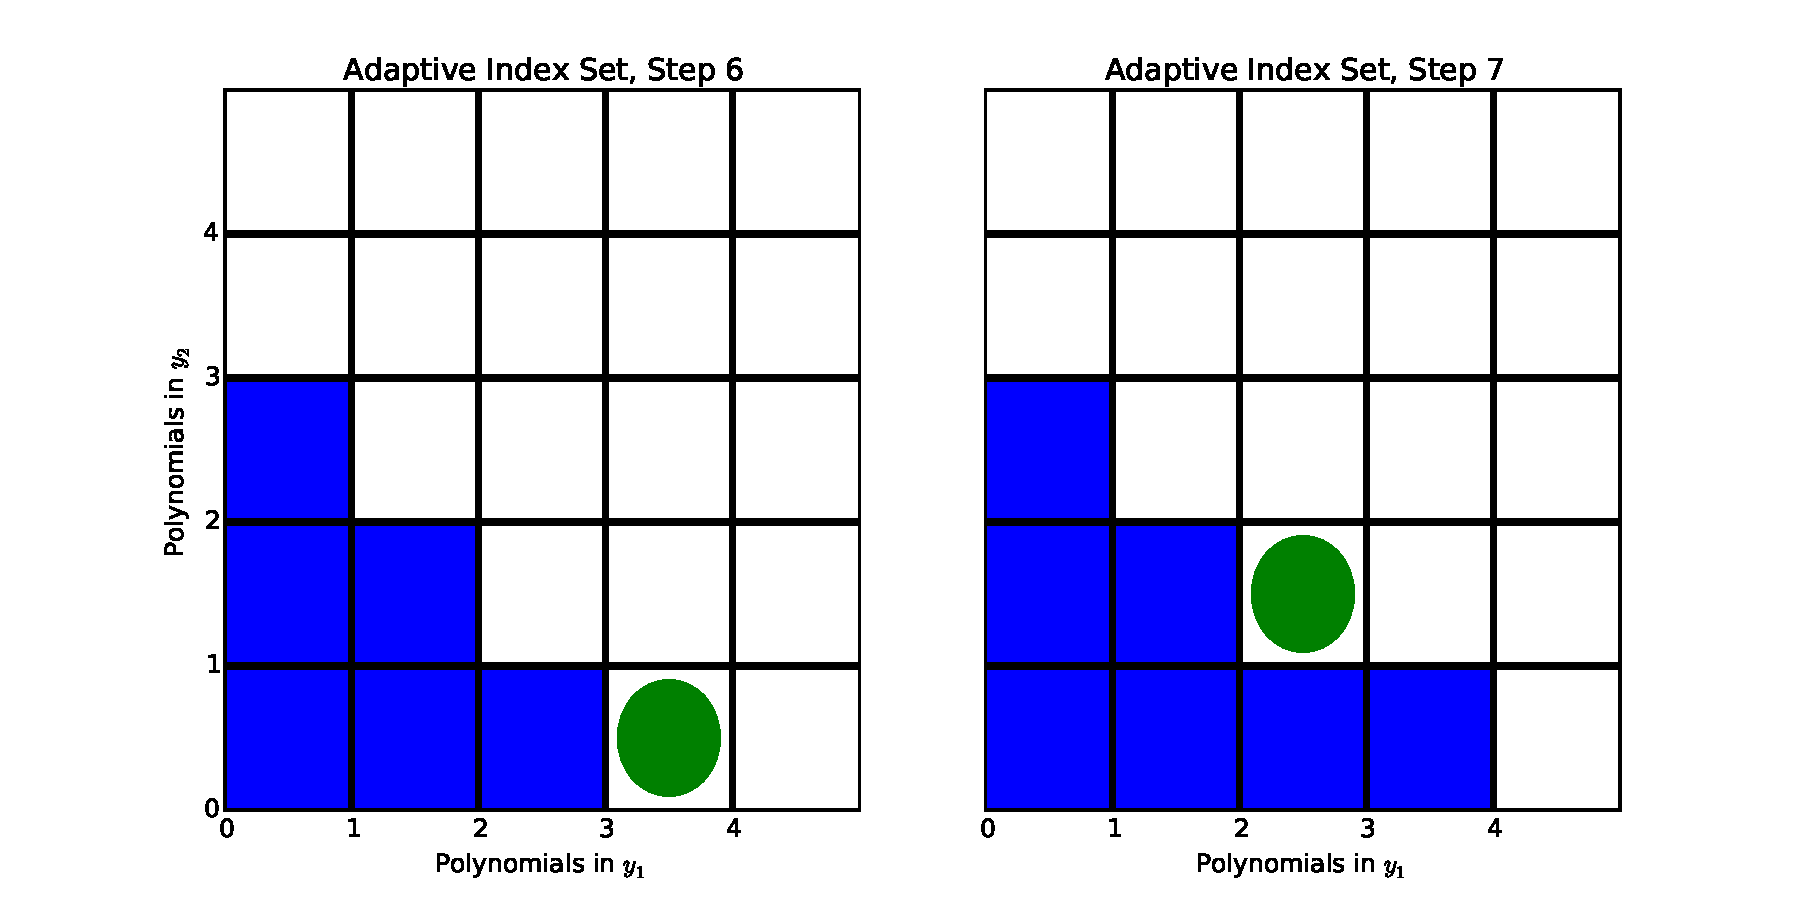
\includegraphics[width=\linewidth]{asc_step}
  \caption{Adaptive Sparse Grid Step}
  \label{fig:asg step}
\end{figure}
\begin{figure}[H]
  \centering
  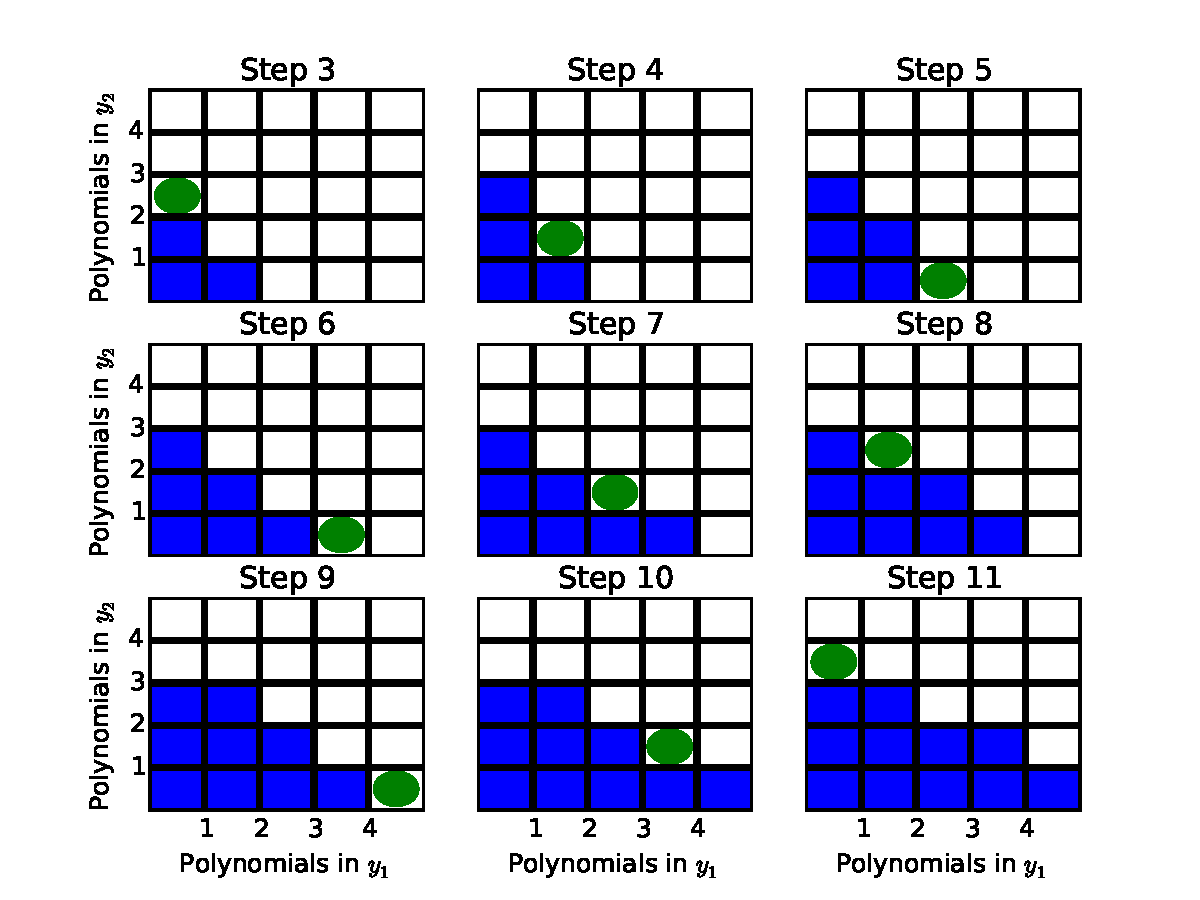
\includegraphics[width=0.7\linewidth]{asc_block}
  \caption{Adaptive Sparse Grid Progression}
  \label{fig:asg block}
\end{figure}

There are, however, some weak points in this algorithm.  First, the current algorithm has no predictive method
to determine the next polynomial index to include in the set; instead, it evaluates each potential index and
selects the one with the most impact \cite{Ayres}.  This is somewhat inefficient, because of SCgPC representations created
that are not used in the final product.  One improvement we make to this algorithm is to predict the impact of
un-evaluated polynomials based on the impact of predecessors.

In order to predict the most valuable polynomial to add to the expansion during an adaptive search, we first
identify a metric for value.  Because our interest is in second-order statistics, and the variance of the
polynomial expansions is the sum of the polynomial expansion coefficients, we consider the \emph{impact}
$\eta_k$ of a polynomial to be the square of its polynomial expansion coefficient,
\begin{equation}\label{eq: act poly impact}
  \eta_k = u_k^2.
\end{equation}
To estimate the impact of a polynomial whose coefficient is not yet calculated, we consider the average of the
preceeding polynomials.  That is, for a polynomial $k=(3,2,4)$ we average the impacts of $(2,2,4)$, $(3,1,4)$,
and $(3,1,3)$,
\begin{equation}\label{eq: poly impact}
  \tilde \eta_k = \frac{1}{N-j}\sum_{n=1}^N \eta_{k-e_n},
\end{equation}
where $\tilde \eta_k$ is the estimated impact of polynomial $k$, $e_n$ is a unit vector in dimension $n$, and
for every entry where $k-e_n$ would reduce one index to less than 0, it is skipped and $j$ is incremented by
one.  In this way any polynomial with some missing predecessors is still averaged appropriately with all
available information.  While occasionally this prediction algorithm may be misled, in general it saves
significantly over the previous algorithm.

Another weakness of the adaptive sparse grid algorithm is that 
there are certain types of models for which the adaptive algorithm will stall, converge too early, or
similarly fail.  For instance, if the partial derivative of the model with respect to any of the
input dimensions is zero when evaluated at the mean point (but nonzero elsewhere), the algorithm will falsely
converge prematurely, as adding additional polynomial orders to the input in question will not change the
value of the model at the mean point.  For example, consider a model
\begin{equation}
  f(a,b) = a^3b^3,
\end{equation}
with both $a$ and $b$ uniformly distributed on [-1,1].  We note the partial derivatives with respect to either
input variable evaluated at the central point (0,0) are zero.  The first polynomial index set point to
evaluate is zeroth-order in each dimension, [0,0].  We distinguish input domain points from polynomial index
set points by using parenthesis for the former and square brackets for the latter. The quadrature point to
evaluate this polynomial coefficient is (0,0), which, when evaluated, gives $f(0,0)=0$.  The next polynomial
index set combinations are [1,2] and [2,1].  For [1,2], the quadrature points required are
(0,$\pm\sqrt{1/3}$).  This evaluates to $f(0,\pm\sqrt{1/3})=0$, as well.  Because of symmetry, we obtain the
same result of [2,1].  According to our algorithm, because our old value was 0, and the sum of the new
contributions is 0, we have converged; however, we know this is false convergence.  While we expect few
applications for SCgPC to exhibit these zero partial derivatives in the input space, it is a limitation to be
aware of.  An argument can be made that, since lower-order polynomials correspond to lower-energy modes of the
modeled physics, it is expected that higher-order polynomials should rarely contribute to an accurate
expansion unless lower-order polynomials contribute as well.
